\begin{frame}[t]{Background}
    
\begin{itemize}
\begin{columns}
 \begin{column}{0.35\textwidth}
  \item 2D/1D method was developed by researchers at Korea Atomic Energy 
  Research Institute (KAERI) \cite{3DHetWholeCoreTransPlanarMOC,DeCARTTheoryManual,MethodsAndPerformanceOfDecart}
  \begin{itemize}
      \item Takes advantage of reactor geometry
      \item High fidelity transport radially with faster, lower order method axially
  \end{itemize}
\end{column}
\begin{column}{0.55\textwidth}
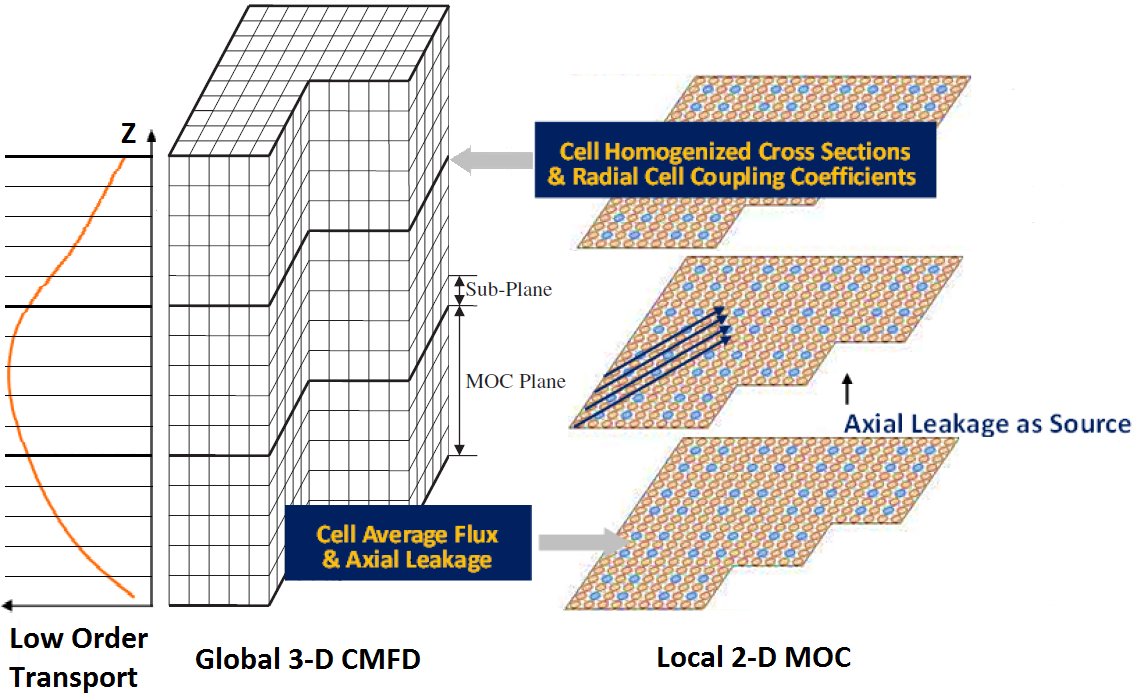
\includegraphics[width=\columnwidth]{../figs/2d1d-subplane.png}
\vfill  
\end{column}
\end{columns}
\begin{columns}
\begin{column}{0.95\textwidth}
\item Newer 2D/1D code MPACT, jointly developed by University of Michigan and Oak Ridge National Laboratory, is used for this work
\end{column}
\end{columns}
\end{itemize} 
  
\end{frame}

%%%%%%%%%%%%%%%%%%%%%%%%%%%%%%%%%%%%%%%%%%%%%%%%%%%%%%%%%%%%%%%%%%%%%%%%%%%%%%%%%

\begin{frame}[t]{Radial Equations}
    
    \begin{itemize}
      \item Average transport equation axially from $z_{k-\frac{1}{2}}$ to 
      $z_{k+\frac{1}{2}}$
      \item Assume cross sections are axially constant in region of integration
    \end{itemize}
    \begin{dmath*}
        {\Omega_x\frac{\partial \psi_{g}^Z}{\partial x} + 
        \Omega_y\frac{\partial \psi_{g}^Z}{\partial y}} + 
        {\Sigma_{tr,g}\left(x,y\right)\psi_{g}^Z\left(x,y,\bm\Omega\right)} = 
        {q_{g}^Z\left(x,y,\bm \Omega\right)} + 
        {L_{g}^Z\left(x,y,\Omega_z\right)}
    \end{dmath*}
    \begin{dmath*}
        {q_{g}^Z\left(x,y,\bm \Omega\right)} = 
        {\frac{1}{4\pi}\sum_{g'=1}^{G}\intop_{4\pi}\Sigma_{s,g'\rightarrow 
        g}^Z\left(x,y,\bm\Omega'\cdot\bm\Omega\right)\psi_{g'}^Z\left(x,y,\bm\Omega'\right)d\Omega'}
         + {\frac{1}{k_{eff}}\frac{\chi_{g}^Z}{4\pi}\sum_{g'=1}^G\intop_{4\pi} 
        \nu\Sigma_{f,g'}^Z\left(x,y\right)\psi_{g'}^Z\left(x,y,\bm\Omega'\right)d\Omega'}
         + {\frac{Q_{g}^Z\left(x,y\right)}{4\pi}}
    \end{dmath*}
    \begin{align*}
    L_{g}^Z\left(x,y,\Omega_z\right) &= \frac{\Omega_z}{\Delta z_k}\left(\psi_{g,z_{k-\frac{1}{2}}} - \psi_{g,z_{k+\frac{1}{2}}}\right) \approx \frac{J_{g,z_{k-\frac{1}{2}}} - J_{g,z_{k+\frac{1}{2}}}}{4\pi\Delta z_k}
    \end{align*}
    
\end{frame}

%%%%%%%%%%%%%%%%%%%%%%%%%%%%%%%%%%%%%%%%%%%%%%%%%%%%%%%%%%%%%%%%%%%%%%%%%%%%%%%%%

\begin{frame}[t]{Axial Equations}

\begin{itemize}
  \item Average transport equation over x from $x_{i-\frac{1}{2}}$ to 
  $x_{i+\frac{1}{2}}$ and over y from $y_{j-\frac{1}{2}}$ to $y_{j+\frac{1}{2}}$
  \item Assume cross sections are radially constant in region of integration
\end{itemize}
\begin{dmath*}
{\Omega_z \frac{\partial \psi_{g}^{XY}}{\partial z}} + 
{\Sigma_{tr,g}^{XY}\left(z\right)\psi_{g}^{XY}\left(z,\bm\Omega\right)} = 
q_{g}^{XY}\left(z,\bm\Omega\right) + 
{L_{g}^{XY}\left(z,\Omega_x,\Omega_y\right)}
\end{dmath*}
\begin{equation*}
L_{g}^{XY}\left(z,\Omega_x,\Omega_y\right) \approx 
{\frac{J_{g,x_{i-\frac{1}{2}},y_j} - 
  J_{g,x_{i+\frac{1}{2}},y_j}}{4\pi\Delta x_i}} +
\frac{J_{g,x_i,y_{j-\frac{1}{2}}} - J_{g,x_i,y_{j+\frac{1}{2}}}}{4\pi\Delta 
y_j}
\end{equation*}

\end{frame}

%%%%%%%%%%%%%%%%%%%%%%%%%%%%%%%%%%%%%%%%%%%%%%%%%%%%%%%%%%%%%%%%%%%%%%%%%%%%%%%%%

\begin{frame}[t]{Calculation Flow}

\begin{columns}
  \begin{column}{0.6\textwidth}
    \begin{itemize}
      \item 3D CMFD \cite{SmithCMFDOrig}
      \begin{itemize}
        \item Determines global flux shape to scale fine mesh solution
        \item Calculates radial currents for 1D axial solver
      \end{itemize}
      \item 1D NEM-SP$_3$ \cite{SPnEquations,finnemann1977RodCuspingOrigMention}
      \begin{itemize}
        \item Calculates improved axial currents for 2D solver
      \end{itemize}
      \item 2D MOC \cite{AskerMOCOrig1972,HalsallMOCOrigCACTUS1980}
      \begin{itemize}
        \item Solves for fine mesh scalar flux
        \item Calculates updated radial currents for CMFD calculation
      \end{itemize}
    \end{itemize}
  \end{column}
\begin{column}{0.4\textwidth}
  \begin{figure}[h]
    \centering
    \resizebox{!}{0.7\textheight}{\begin{tikzpicture}[node distance=2cm]

% Begin
\node (start) [startstop] {Start};
\node (init) [io, right of=start, xshift=2.0cm] {Input, Initialize Solution};

% CMFD
\node (CMFD) [process, below of=init] {CMFD Eigenvalue Calculation};

% Nodal
\node (Nodal) [process, below of=CMFD] {Axial P$_3$ Calculation};

% MOC
\node (MOC) [process, below of=Nodal] {2D MOC Sweeps};

% Finish
\node (convCheck) [decision, below of=MOC, yshift=-1.5cm] {Fission Source, k-eff Converged?};
\node (out) [io, below of=convCheck,yshift=-1.5cm] {Output};
\node (stop) [startstop, right of=out, xshift=2.0cm] {Stop};

% Basic Arrows
\draw [arrow] (start) -- (init);
\draw [arrow] (init) -- (CMFD);
\draw [arrow] (CMFD) -- (Nodal);
\draw [arrow] (Nodal) -- (MOC);
\draw [arrow] (MOC) -- (convCheck);
\draw [arrow] (out) -- (stop);

% Fancy Arrows
\draw [arrow] (convCheck) -- node[anchor=west] {yes} (out);
\draw [arrow] (convCheck) -| node[anchor=north] {no} ([xshift=1.5cm]Nodal.east) |- (CMFD);

\end{tikzpicture}}
  \end{figure}
\end{column}
\end{columns}

\end{frame}

%%%%%%%%%%%%%%%%%%%%%%%%%%%%%%%%%%%%%%%%%%%%%%%%%%%%%%%%%%%%%%%%%%%%%%%%%%%%%%%%%

\begin{frame}[t]{3D CMFD}
    
        \begin{itemize}
          \item Diffusion-based acceleration performed on coarse mesh
          \item $\hat{D}$ coupling coefficients enforce consistency between diffusion and transport solutions
          \begin{equation*}\scriptstyle
          \hat{D}_{g,s} = \frac{J_{g,s}^{trans,k-1} + 
            \tilde{D}_{g,s}\left(\phi_{g,p}^{diff,k} - 
            \phi_{g,m}^{diff,k}\right)}{\left(\phi_{g,p}^{trans,k} + 
            \phi_{g,m}^{diff,k}\right)}
          \end{equation*}
          \item Coarse mesh solution projected to fine mesh solution, preserving MOC radial shape and CMFD volume-averaged flux
          \begin{equation*}\scriptstyle
          \phi_{g,j}^{MOC,k} = \frac{\phi_{g,i}^{CMFD,k}}{\phi_{g,i}^{CMFD,k-1}} \phi_{g,j}^{MOC,k-1}
          \end{equation*}
          \item Subplane scheme is used to capture subplane axial flux shapes
        \end{itemize}
    
\end{frame}

%%%%%%%%%%%%%%%%%%%%%%%%%%%%%%%%%%%%%%%%%%%%%%%%%%%%%%%%%%%%%%%%%%%%%%%%%%%%%%%%%

\begin{frame}[t]{1D SP$_3$-NEM}
    
    \begin{columns}
      \begin{column}{0.6\textwidth}
        \begin{itemize}
          \item SP$_3$ \cite{SPnEquations} used to handle angular shape 
          \begin{dmath*}\scriptstyle
            {-\bm{\nabla} \cdot D_{0,g} \left(\bm x\right) \bm \nabla 
            \Phi_{0,g}\left(\bm x\right) + \left[\Sigma_{tr,g}\left(\bm 
            x\right) - \Sigma_{s0,g}\left(\bm 
            x\right)\right]\Phi_{0,g}\left(\bm x\right)} = {Q_g\left(\bm 
            x\right) + 2\left[\Sigma_{tr,g}\left(\bm x\right) - 
            \Sigma_{s0,g}\left(\bm x\right)\right]\Phi_{2,g}\left(\bm 
            x\right)}
          \end{dmath*}
          \begin{dmath*}\scriptstyle
            {-\bm{\nabla} \cdot D_{2,g} \left(\bm x\right) \bm \nabla 
            \Phi_{2,g}\left(\bm x\right) + \left[\Sigma_{tr,g}\left(\bm 
            x\right) - \Sigma_{s2,g}\left(\bm 
            x\right)\right]\Phi_{2,g}\left(\bm x\right)} = 
            {\frac{2}{5}\left\lbrace \left[\Sigma_{tr,g}\left(\bm x\right) - 
            \Sigma_{s0,g}\left(\bm x\right)\right]\left[\Phi_{0,g}\left(\bm 
            x\right) - 2\Phi_{2,g}\left(\bm x\right)\right] - Q_g\left(\bm 
            x\right) \right\rbrace}
          \end{dmath*}
          \item NEM \cite{finnemann1977RodCuspingOrigMention} used to handle spatial shape
          \begin{equation*}\scriptstyle
          Q\left(\xi\right) = \sum_{i=0}^2 q_i P_i\left(\xi\right)\ , \quad 
          \phi\left(\xi\right) = \sum_{i=0}^4 \phi_i P_i\left(\xi\right)
          \end{equation*}
          \begin{equation*}\scriptstyle
          \intop_{-1}^1 P_n\left(\xi\right) 
          \left(-\frac{D}{h^2}\frac{d^2}{d\xi^2}\phi\left(\xi\right) + \Sigma_r 
          \phi\left(\xi\right) - Q\left(\xi\right)\right)d\xi = 0,\ n=0,1,2
          \end{equation*}
          \begin{equation*}\scriptstyle
          \phi_L\left(1\right) = \phi_R\left(-1\right)\ , \quad 
          J_L\left(1\right) = J_R\left(-1\right)
          \end{equation*}
        \end{itemize}
      \end{column}
    \begin{column}{0.4\textwidth}
      \begin{figure}[h]
        \centering
        \resizebox{!}{0.5\textheight}{\begin{tikzpicture}[node distance=2cm]

% Begin
\node (start) [startstop] {Start};

% Nodal
\node (radialTL) [process, right of=start, xshift=2.5cm] {Calculate radial transverse leakage source};
\node (sp3-0) [process, below of=radialTL] {Solve 0th moment equation};
\node (sp3-2) [process, below of=sp3-0] {Solve 2nd moment equation};
\node (convCheck) [decision, below of=sp3-2, yshift=-1.5cm] {Converged?};

% Stop
\node (stop) [startstop, right of=convCheck, xshift=2.5cm] {Stop};

% Basic Arrows
\draw [arrow] (start) -- (radialTL);
\draw [arrow] (radialTL) -- (sp3-0);
\draw [arrow] (sp3-0) -- (sp3-2);
\draw [arrow] (sp3-2) -- (convCheck);
\draw [arrow] (convCheck) -- node[anchor=north] {yes} (stop);

% Fancy Arrows
\draw [arrow] (convCheck) -| node[anchor=north] {no} ([xshift=-1.5cm]sp3-2.west) |- (sp3-0);

\end{tikzpicture}}
      \end{figure}
    \end{column}
    \end{columns}
    
\end{frame}

%%%%%%%%%%%%%%%%%%%%%%%%%%%%%%%%%%%%%%%%%%%%%%%%%%%%%%%%%%%%%%%%%%%%%%%%%%%%%%%%%

\begin{frame}[t]{2D MOC}

    \begin{itemize}
      \item Solve along a specific direction $\Omega_n$ to reduce the problem from a PDE to an ODE that can be solved analytically
      \begin{equation*}\scriptstyle
      \frac{\partial \psi_{g,n}}{\partial s} + \Sigma_{t,g}\left(\bm r_0 + 
      s\bm\Omega_n\right)\psi_{g,n}\left(\bm r_0 + s\bm\Omega_n\right) = 
      q_{g,n}\left(\bm r_0 + s\bm\Omega_n\right)
      \end{equation*}
      \begin{dmath*}\scriptstyle
        {\psi_{g,n}\left(\bm r_0 + s\bm\Omega_n\right) = \psi_{g,n}\left(\bm 
        r_0\right)\exp{\left(-\intop_0^s \Sigma_{t,g}\left(\bm r_0 + 
        s'\bm\Omega_n\right)ds'\right)}} + {\intop_0^s q_{g,n}\left(\bm r_0 + 
        s'\bm\Omega_n\right)\exp{\left(-\intop_0^{s'} \Sigma_{t,g}\left(\bm r_0 
        + s''\bm\Omega_n\right)ds''\right)}ds'}
      \end{dmath*}
  \item Assume flat source, cross section along track with 
length $L_j$ and spacing $\delta x$
\begin{align*}\scriptstyle
\psi^{out}_{g,i,n,j} &\scriptstyle = \psi^{in}_{g,i,n,j}e^{-\Sigma_{t,g,i} 
    L_j} + \frac{q_{g,i,n}}{\Sigma_{t,g,i}}\left(1 - 
e^{-\Sigma_{t,g,i}L_j}\right) \\\scriptstyle
\overline{\psi}_{g,i,n,j} &\scriptstyle = 
\frac{q_{g,n,i}}{\Sigma_{t,g,i}} + \frac{1 - e^{-\Sigma_{t,g,i} 
        L_j}}{L_j\Sigma_{t,g,i}}\left(\psi^{in}_{g,i,n,j} - 
\frac{q_{g,n,i}}{\Sigma_{t,g,i}}\right) \\\scriptstyle
\overline{\psi}_{g,i,n} &\scriptstyle = \frac{\sum_j 
    \overline{\psi}_{g,i,n,j} \delta x L_j}{\sum_j \delta x L_j}
\end{align*}
    \end{itemize}

\end{frame} 

%%%%%%%%%%%%%%%%%%%%%%%%%%%%%%%%%%%%%%%%%%%%%%%%%%%%%%%%%%%%%%%%%%%%%%%%%%%%%%%%%

\begin{frame}[t]{2D MOC}
  
  \begin{columns}
    \begin{column}{0.55\textwidth}
      \begin{itemize}
        \item Perform ray tracing and store segment information up front
        \item Set up scattering, fission, and axial transverse leakage sources
        \begin{itemize}
            \item Multi-group sweeping
          \item 1-group sweeping
        \end{itemize}
        \item Parallel Decomposition
        \begin{itemize}
          \item Spatial (Planar and Radial)- MPI
          \item Angle - MPI
          \item Ray - OpenMP
        \end{itemize}
      \end{itemize}
    \end{column}
    \begin{column}{0.45\textwidth}
      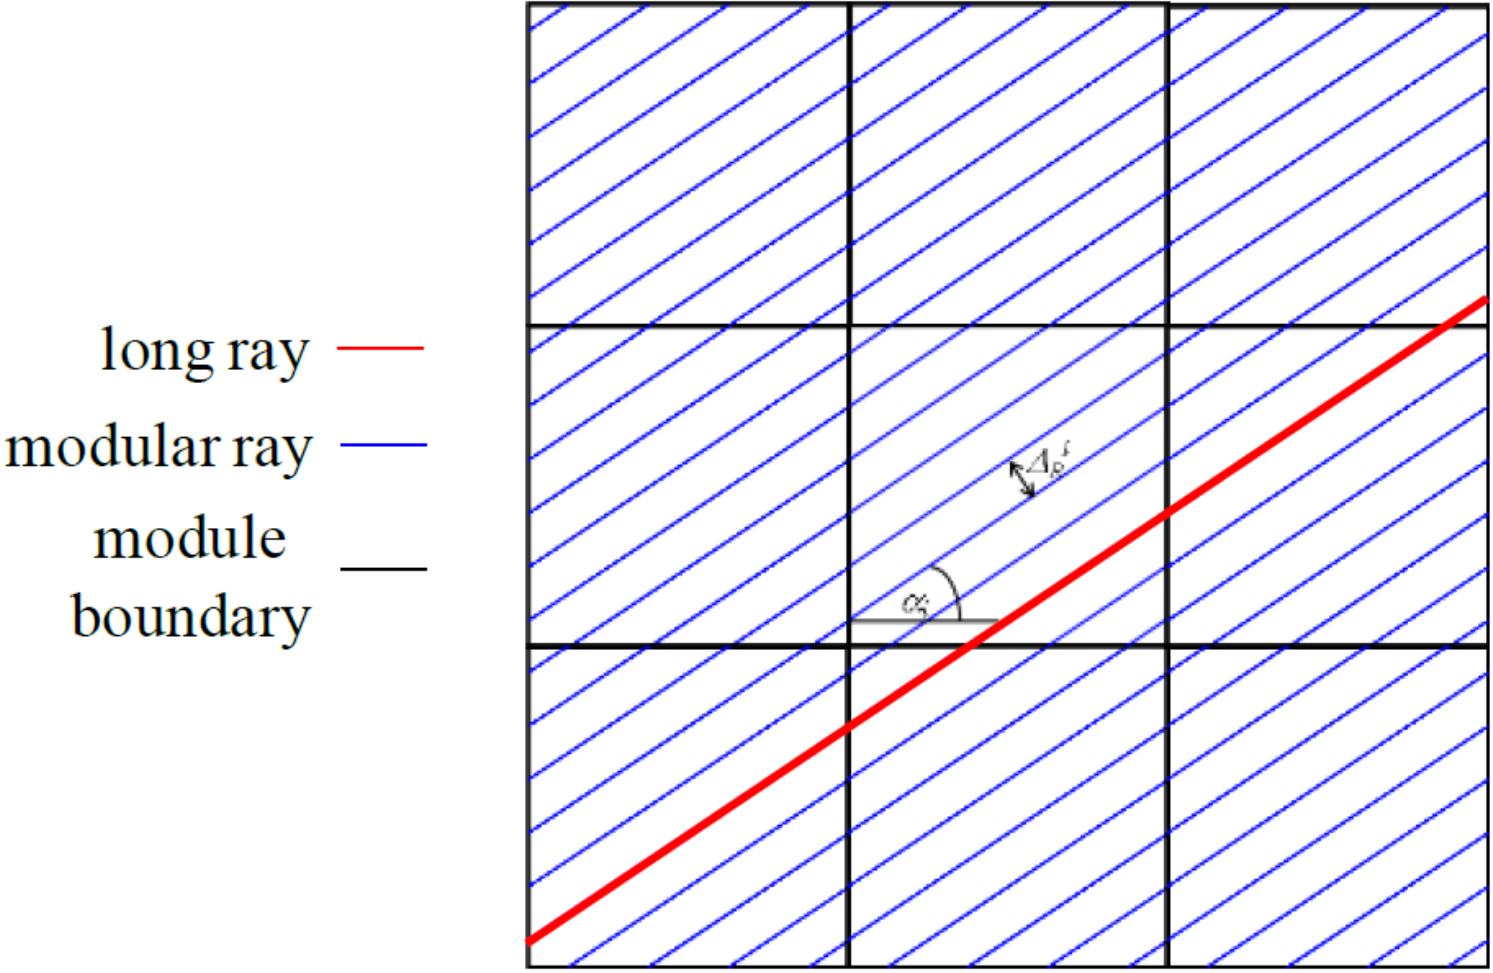
\includegraphics[width=\columnwidth]{modular_rays.png}
    \end{column}
  \end{columns}

\end{frame}